\documentclass[a4paper, 11pt]{article}
\setlength{\topmargin}{-.5in}
\setlength{\textheight}{9in}
\setlength{\oddsidemargin}{.100in}
\setlength{\textwidth}{6.25in}
\usepackage [dutch] {babel}
\usepackage{graphicx}
\usepackage{amsmath}
\usepackage{fullpage}
\usepackage{listings}
\usepackage{color}
\usepackage{soul}
\usepackage{gensymb}
\usepackage{caption}
\usepackage{subcaption}

\begin{document}

\begin{titlepage}
\title{Ontwerp van Software Systemen}
\author{}
\end{titlepage}



\maketitle
\newpage
\tableofcontents
\pagebreak

\section*{Inleiding}

% Een inleiding: beschrijf hierin jullie algemene impressie van het systeem, de manier waarop
% jullie de analyse hebben aangepakt, etc.

In dit project moeten we JUnit ontleden via analyse tools die JUnit gaan visualiseren. JUnit is een testing en regressie testing framework in Java. Om beter de linken tussen de klassen te begrijpen werd er gebruik gemaakt van \emph{X-Ray} \cite{X-Ray} en \emph{AgileJ Structureviews} \cite{AgileJ Structureviews}. Hierna werd voor verdere analyse gebruik gemaakt van \emph{Design Pattern Detection Tool} \cite{Design Pattern Detection Tool} en \emph{CodeCity} \cite{CodeCity}. Voor de visualisatie van de klassendiagrammas en sequence diagrams werd er gebruik gemaakt van \emph{Visual Paradigm}.


\section{Ontwerpdocumentatie}

De klasse die de main methode bevat in het JUnit project is JUnitCore. JUnitCore is een facade voor het uitvoeren van testen. Via de run() methoden kunnen testen worden uitgevoerd. JUnitCore gebruikt de klasse Runner via de methode run(runner) die niet mag worden uitgevoerd. Deze wordt gebruikt bij het testen. De runner test en verwittigd de RunNotifier als er interessante gebeurtenissen voorvallen. 





\section{Evaluatie van het ontwerp}

%Een evaluatie van het ontwerp. Wat zijn sterke en zwakke punten van het ontwerp. Bespreek
%ook het gebruik (of het niet-gebruik) van patronen. Geef opnieuw sterke en zwakke punten
%van het ontwerp op dit vlak.

\section{Beschrijving van de analyse tools en evaluatie hiervan}

Voor de analyse van JUnit werden er vier analyse tools gebruikt. De verschillende tools zijn \emph{X-ray} \cite{X-Ray}, \emph{AgileJ Structureviews} \cite{AgileJ Structureviews} , \emph{Design Pattern Detection Tool} \cite{Design Pattern Detection Tool} en \emph{InFusion Hydrogen}. Om \emph{X-Ray} beter de begrijpen werd er ook nog gekeken naar \emph{CodeCity} \cite{CodeCity}.

\begin{description}

\item \emph{X-Ray}: \emph{X-Ray} is een visualisatie tool die de complexiteit van de klassen weergeeft. Figuur \ref{fig:X-Ray} geeft dit weer. De rechthoeken geven de klassen weer. De lengte van een rechthoek geeft het aantal methodes weer en de breedte de  ... . Overerving wordt weergegeven via een boomstructuur. Met X-Ray kan je ook opzoeken wie de parents zijn van een klasse of de childs. Via kleuren geven ze ook het typpe klasse mee: Abstract, Concrete, Interface en Internal Classes. X-Inkomende dependencies liet X-Ray niet zien, alleen uitgaande dependecies.   

\begin{figure}[hb!]
	\centering
	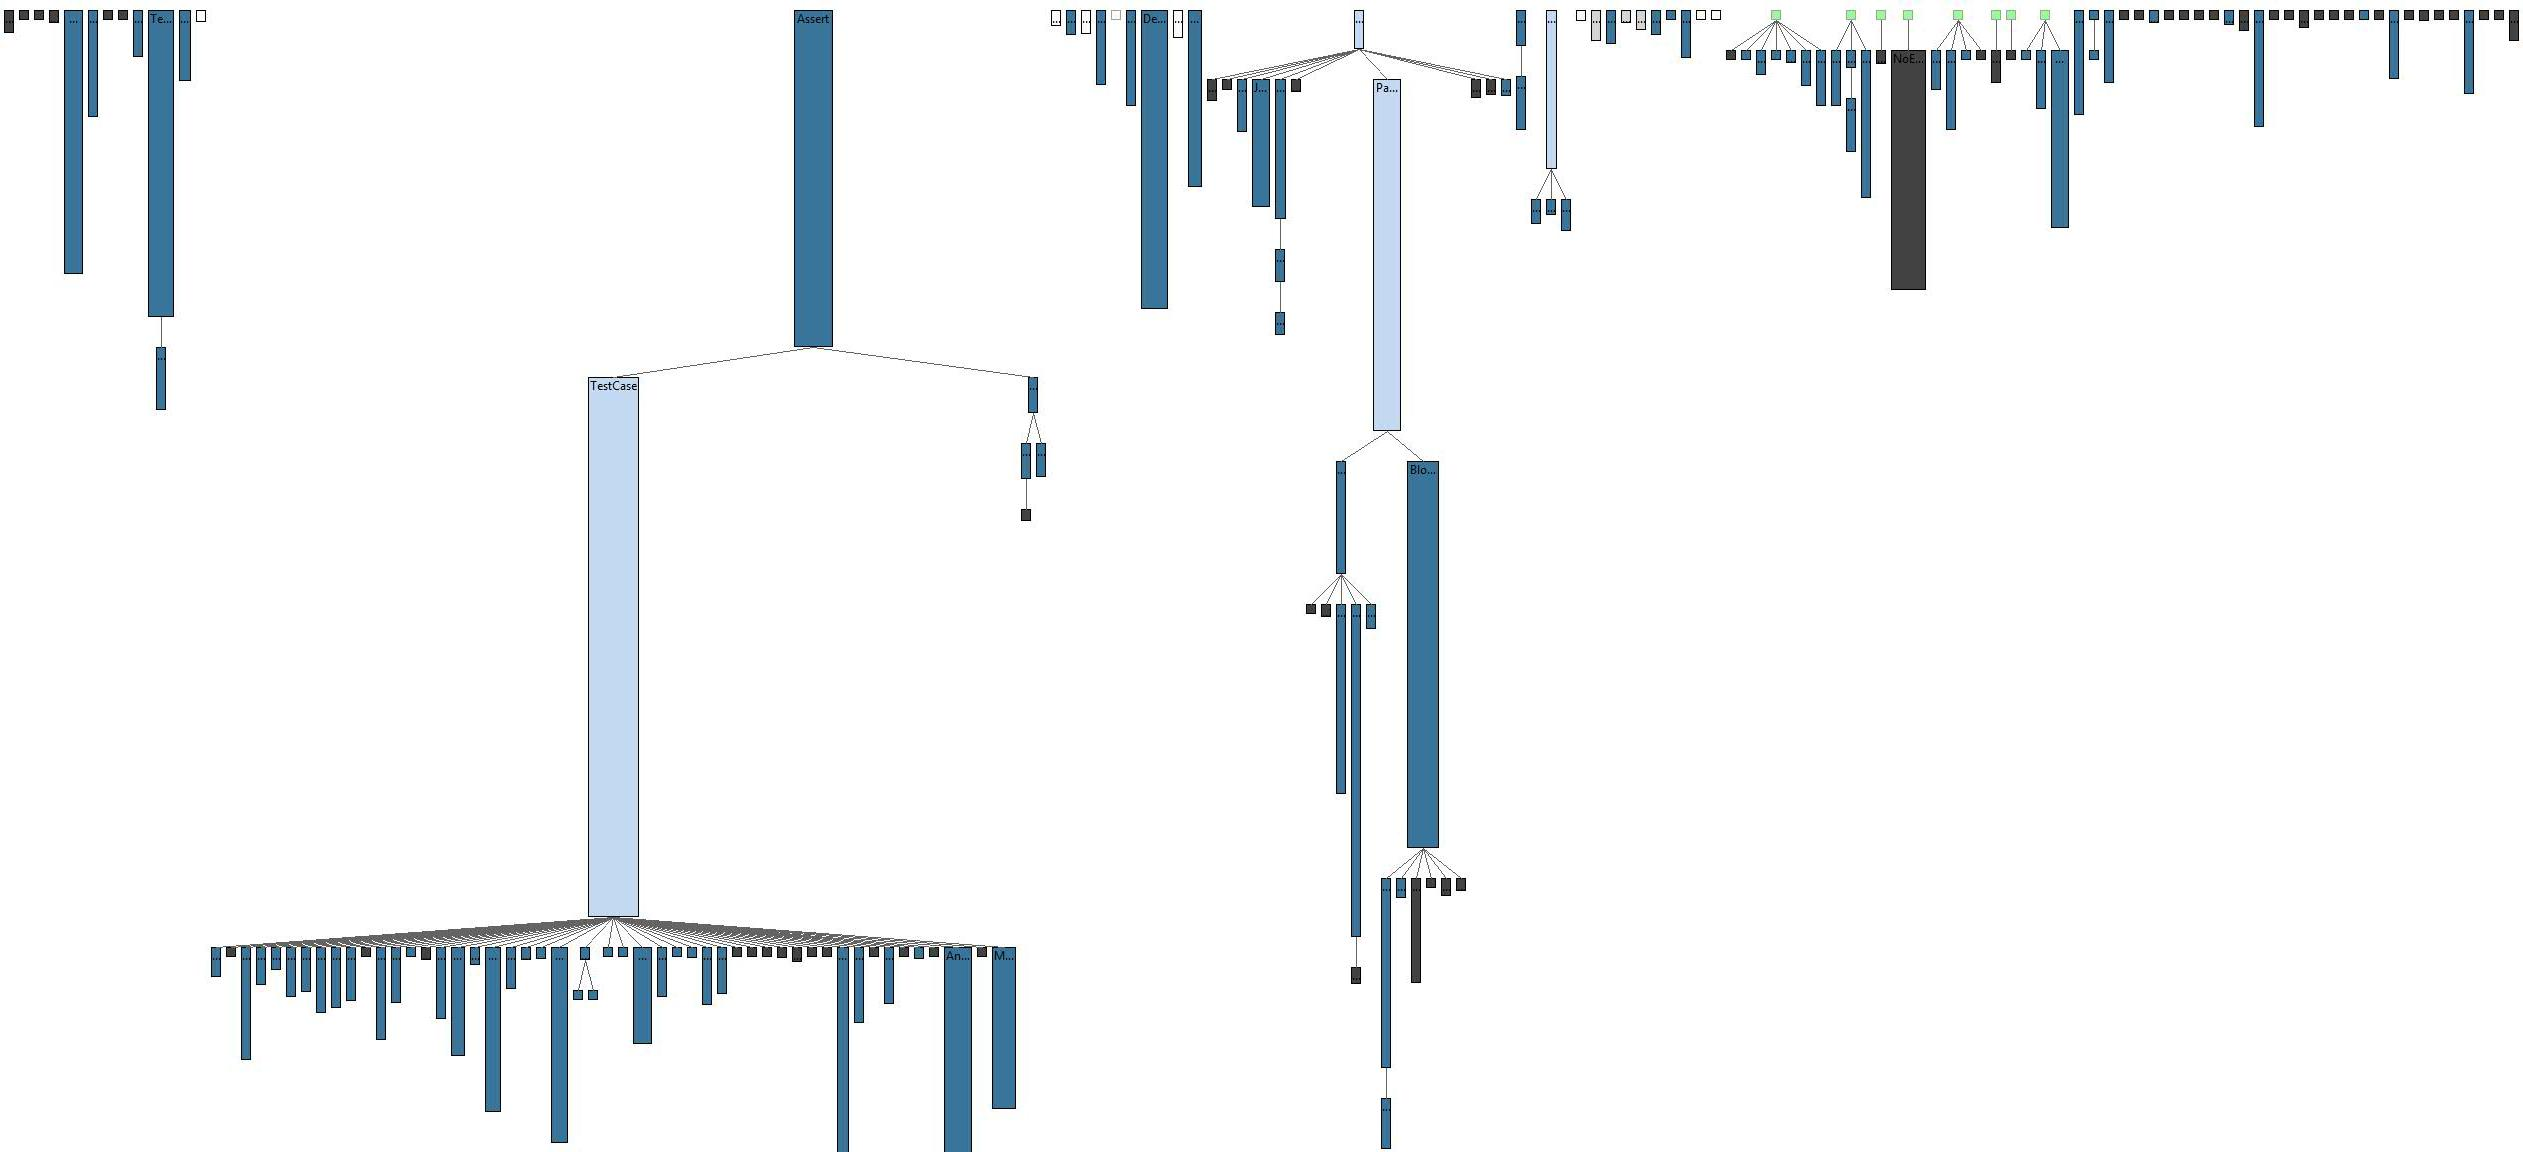
\includegraphics[width=0.52\textwidth]{XRayComplexity}
	\caption{X-Ray: Complexiteit}
	\label{fig:X-Ray}
\end{figure}

\item \emph{AgileJ Structureviews}: AgileJ Structureviews is een visualistatie tool die klassendiagrammas kan genereren. Figuur \label{fig:AgileJklassendia} geeft een voorbeeld visualisatie weer van een klassendiagramma die gegenereerd is via AgileJ.


\begin{figure}[hb!]
	\centering
	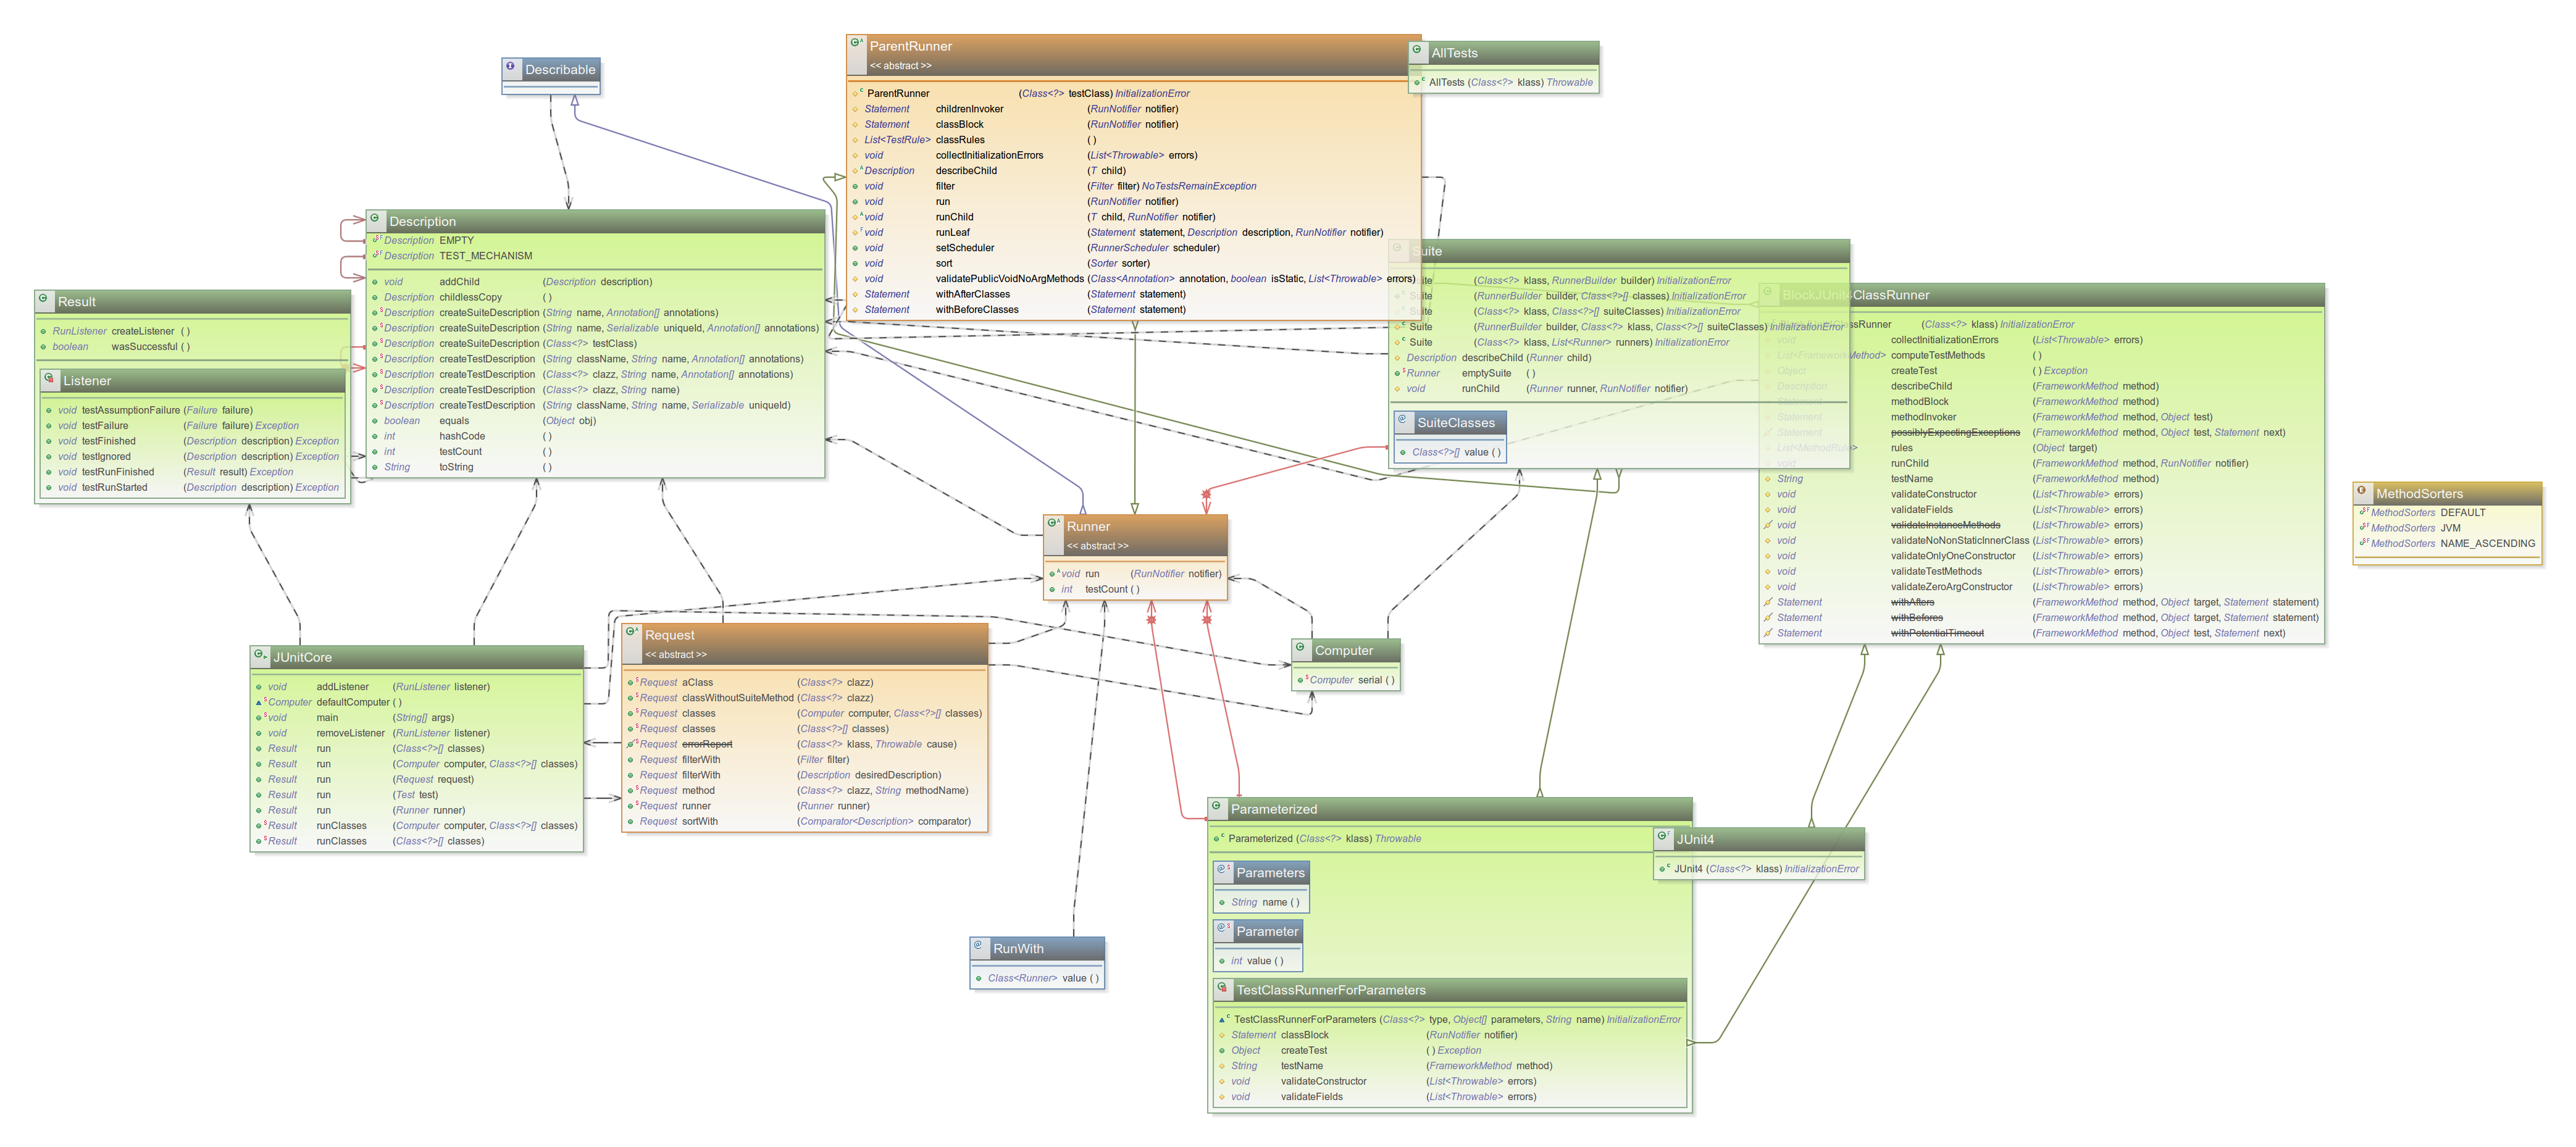
\includegraphics[width=0.52\textwidth]{AgileJKlassendiagramma}
	\caption{AgileJ Sturcutureviews: klassendiagramma}
	\label{fig:AgileJKlassendia}
\end{figure}

\item \emph{Design Pattern Detection Tool}: Design Pattern Detection Tool is een tool die het programma gaat checken op bepaalde patterns.




\end{description}


\section{Analyse tools en belangrijke resultaten}
Agilj filters gebruikt, Codecity, Xray
Statements wordt gebruikt om alle annotaties uit te voeren
.runner en .runners

\section{Evaluatie testen}

\section{Samenvatting}

\section{projectbeheer}

Wij zijn vrij laat begonnen aan het project omdat onze groep nog niet samengesteld was in het begin van de eerste week. 


\newpage
\begin{flushleft}
\begin{thebibliography}{4}

\bibitem{X-Ray}
\emph{X-Ray}
\begin{scriptsize}
geraadpleegd op 11/10/2013 via: \mbox{http://xray.inf.usi.ch/xray.php} en \mbox{https://marketplace.eclipse.org/content/x-ray-software-visualization}
\end{scriptsize}

\bibitem{AgileJ Structureviews}
\emph{AgileJ Structureviews}
\begin{scriptsize}
geraadpleegd op 11/10/2013 via: \mbox{http://www.agilej.com/}
\end{scriptsize}

\bibitem{Design Pattern Detection Tool}
\emph{Design Pattern Detection Tool}
\begin{scriptsize}
geraadpleegd op 15/10/2013 via: \mbox{http://java.uom.gr/~nikos/pattern-detection.html} versie  Design Pattern detection Tool (version 4.5 - build 28/05/2010)
\end{scriptsize}

\bibitem{CodeCity}
\emph{CodeCity}
\begin{scriptsize}
geraadpleegd op 9/10/2013 via: \mbox{http://www.inf.usi.ch/phd/wettel/codecity.html} 
\end{scriptsize}

\end{thebibliography}
\end{flushleft}

\end{document}



